\section{Effect trees}
\label{section:trees}

The general scenario this paper addresses is that of a programming language whose programs may perform effects as they compute. In this paper, we assume that the available effects are  specified 
by  an \emph{effect signature}: a set $\Sigma$ of operation symbols, each with an associated finite arity. We call the operations in $\Sigma$ \emph{effect operations}. This setting is explicitly that of \cite{plotkin2001adequacy}.
More general effect signatures appear in the literature, e.g., allowing parameterised operations and infinite arities
\cite{gom}  [[OTHER REFERENCES]]. The technical development in this paper can be generalised to such
more general signatures. Since, however, the main running example considered in this paper has only binary operations, we restrict ourselves to finite arity operations 
for the sake of presentational convenience. %We now present this example.
\begin{example}[Signature for combined probabilistic and non-deterministic choice]
\label{example:prnd}
    Consider a programming language that can perform two effects: probabilistic and nondeterministic choice.
    An appropriate signature for such a language is 
    $\Sigma_{\prnd} = \{ (\prEff,2), (\orEff,2) \}$ containing two binary operations:
    nondeterministic choice $\orEff$, 
    and fair probabilistic choice $\prEff$. (As is well known, in programming languages with general recursion, all computable discrete probability distributions can be 
     simulated using fair probabilistic choice.)
 \end{example}

During the execution of a program with effects, three different situations can arise. Firstly, the computation process may
trigger an effect, represented by some $o \in \Sigma$. The execution will then continue along one of the $n$ possible continuation processes given as arguments to the operation $o$. Secondly, the execution may terminate, 
in which case it may produce a resulting value. 
Thirdly, the execution may continue forever without terminating and without invoking any effects. We call this last situation
 \emph{silent nontermination} to distinguish it from \emph{noisy nontermination}, which occurs
 when the computation process computes for ever while performing an infinite sequence of effects along the way.

The global behaviour of such a program is captured by the notion of an \emph{effect tree}: a  finitely branching tree, whose 
internal nodes represent effect operations, and whose leaves represent either termination with a result, or silent nontermination. The branches of the tree represent potential execution sequences of the program. 
Trees are allowed to be infinitely deep, with their infinite branches representing noisy nontermination.
Such trees were introduced as \emph{infinitary effect values} in  \cite{plotkin2001adequacy}, and used extensively in \cite{gom}, where they are called
\emph{computation trees}. Two example trees, for computations that return natural number values, are drawn in
Figure~\ref{fig:exampletrees} below. The left-hand tree $\orEff (\prEff (1,2), 3)$ represents a program that first makes a nondeterministic choice and then a potential probabilistic choice, with the choices determining the resulting number. In the second tree $\prEff (\orEff (1,3), \orEff (2,3))$, the probabilistic choice is made first, followed by the relevant nondeterministic choice.

\begin{figure}[h]
\small
    \begin{center}
        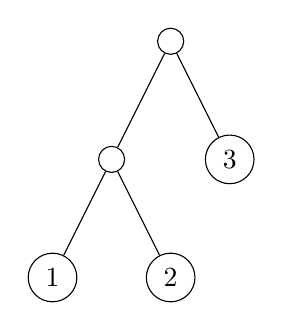
\begin{tikzpicture}
            \node [circle,draw] (z){$\orEff$}
                child { 
                    node [circle,draw] (a) {$\prEff$}
                    child { node[circle,draw] (b) {$1$} } 
                    child { node[circle,draw] (c) {$2$} }
                }
                child {
                    node [circle,draw] (d) {$3$}    
                };
        \end{tikzpicture}
        \hspace*{8ex}
        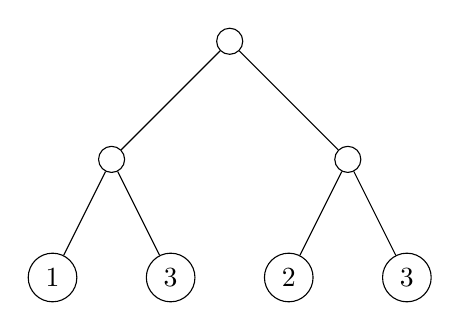
\begin{tikzpicture}[level 1/.style={sibling distance=3cm},
                            level 2/.style={sibling distance=1.5cm}]
            \node [circle,draw] (z){$\prEff$}
                child { 
                    node [circle,draw] (h) {$\orEff$}
                    child { node[circle,draw] (b) {$1$} } 
                    child { node[circle,draw] (c) {$3$} }
                }
                child {
                    node [circle,draw] (g) {$\orEff$}
                    child { node[circle,draw] (e) {$2$} } 
                    child { node[circle,draw] (f) {$3$} }
                };
        \end{tikzpicture}
    \end{center}
%  \begin{equation*}
%        \orEff (\prEff (1,2), 3) \quad \quad \prEff (\orEff (1,3), \orEff (2,3))
 %   \end{equation*}
    \caption{Two effect trees}
    \label{fig:exampletrees}
\end{figure}






\begin{definition}
The set $\Trees(X)$ of \emph{effect trees} with values from  the set $X$ is coinductively defined so that
every tree has one of the following  forms.
\begin{itemize}
\item The root of the tree is labelled with an operation $o \in \Sigma$, and the tree has the form
         $o(t_1, \dots, t_n)$ where $n$ is the arity of $o$ and $t_1, \dots, t_n \in \Trees(X)$; or
\item the tree is a leaf labelled with a value $x \in X$; or
\item the tree is a leaf labelled with $\bot$.
\end{itemize}
\end{definition}
As this is a coinductive definition, $\Trees(X)$ contains trees of both finite and infinite depth.

We define a partial order on  $\Trees(X)$ by
$t_1 \Treeleq t_2$ if and only if $t_2$ can be obtained from $t_1$ by replacing (possibly infinitely many)
$\bot$-leaves appearing in $t_1$ with arbitrary replacement trees (rooted where the leaves were located). With this ordering,  $\Trees(X)$  is an $\omega$-complete 
partial order ($\omega$CPO) with least element $\bot$. Furthermore, by considering it as
a tree constructor,
every operation $o \in \Sigma$  defines a continuous (i.e., $\omega$-continuous) function $o : \Trees(X)^n \to \Trees(X)$, where $n$ is the arity of $o$.
(For notational convenience, we use $o$ for both operation symbol and function. The ambiguity can be resolved from the context.) 

The properties described above state that $\Trees(X)$ is a continuous $\Sigma$-algebra. In general,
a \emph{continuous $\Sigma$-algebra} is a pointed (i.e., with least element) $\omega$CPO $A$ with associated
continuous functions $o_A : A^n \to A$ for every $o \in \Sigma$ of arity $n$. 
As morphisms between continuous $\Sigma$-algebras
$A$ and $B$, we consider functions $h: A \to B$  that are strict (i.e., preserve least element) continuous homomorphisms with respect to the $\Sigma$-algebra structure. 
We refer to such  functions $h: A \to B$ as \emph{continuous homomorphisms}, leaving the strictness property implicit.
We write $\ContAlg_\Sigma$ for the category of continuous $\Sigma$-algebras and continuous homomorphisms.
The characterisation of $\Trees(X)$ below is standard.
%\todo[inline]{[[REFERENCES]]}
\begin{proposition}
$\Trees(X)$ is the free
    continuous $\Sigma$-algebra over the set $X$.
   \begin{center}
        \begin{tikzcd}
            X
            \arrow[r, "f"] 
            \arrow[d, hook, "i"]
            & A \\
            \Trees(X) \arrow[ru, dashrightarrow, "\hat{f}" below]
        \end{tikzcd}
    \end{center}
    That is, for every function $f : X \to A$, where 
    $A$ is a continuous $\Sigma$-algebra,
    there exists a unique continuous homomorphism $$\hat{f} : \Trees(X) \to A$$
    such that $
        f = \hat{f} \circ i $, where $i : X \to \Trees(X)$ is the function mapping every $x \in X$ to the 
        leaf-tree labelled $x$.
 \end{proposition}
 
 We use the above proposition to define a substitution operation on trees. For any tree $t \in \Trees(X)$, 
 every function $f \colon X \to \Trees(Y)$ determines a tree $t[f]$ in $\Trees(Y)$ defined by substitution, \emph{viz}:
 $t[f] ~ := ~ \hat{f}(t)\,$.
 
